\chapter{Definite and Indefinite Integrals}
\label{chp:definite_and_indefinite_Integrals}	

\section{Definite Integrals}

We now turn our attention to using the Fundamental Theorem of Calculus to calculate definite integrals to (in most cases) obtain the area underneath a curve.\\

The \texttt{int()} command allows us to compute integrals (both definite and indefinite) directly. The \texttt{Int()} command allows us to symbolically view the integral, or assign it to a variable to use later for other computations or calculations. Capitalization is important in Maple.

\subsection{The Definite Integral $\displaystyle\int_{-3}^{3}\frac{1}{x^2+1}\, dx$}

\begin{maplegroup}
\begin{mapleinput}
\mapleinline{active}{1d}{f(x) := 1/(1+x\symbol{94}2);
}{}
\end{mapleinput}
\mapleresult
\begin{maplelatex}
\mapleinline{inert}{2d}{f := proc (x) options operator, arrow; 1/(1+x^2) end proc}{\[\displaystyle f\, := \,x\mapsto  \frac{1}{ {x}^{2}+1 }\]}
\end{maplelatex}
\end{maplegroup}
\begin{maplegroup}
\begin{mapleinput}
\mapleinline{active}{1d}{plot(f(x), x=-3..3);
}{}
\end{mapleinput}
\mapleresult
\mapleplot{tutorials/figures/Definite_And_Indefinite_Integralsplot2d1-eps-converted-to.pdf}
\end{maplegroup}

\index{plot!axes intervals}
\index{integral!int!definite}
\index{integral!Int!definite}

We use the \texttt{Int()} command to display the integral, and the \texttt{int()} command to evaluate the integral.

\begin{maplegroup}
\begin{mapleinput}
\mapleinline{active}{1d}{Int(f(x), x=-3..3);
}{}
\end{mapleinput}
\marginnote{Note the capital ``I" in this command. This prevents Maple from automatically evaluating the integral.}
\mapleresult
\begin{maplelatex}
\mapleinline{inert}{2d}{Int(1/(x^2+1), x = -3 .. 3)}{\[\displaystyle \int _{-3}^{3}\! \frac{1}{ {x}^{2}+1 }\,{dx}\]}
\end{maplelatex}
\end{maplegroup}

\begin{maplegroup}
\begin{mapleinput}
\mapleinline{active}{1d}{int(f(x), x=-3..3); evalf(%);
}{}
\end{mapleinput}
\mapleresult
\begin{maplelatex}
\mapleinline{inert}{2d}{2*arctan(3)}{\[\displaystyle 2\,\arctan \left( 3 \right) \]}
\end{maplelatex}
\begin{maplelatex}
\mapleinline{inert}{2d}{2.498091544}{\[\displaystyle  2.498091544\]}
\end{maplelatex}
\end{maplegroup}

\subsection{The Definite Integral $\displaystyle\int_{1}^{10} \ln(x) \, dx$}	

\index{mathematical functions!logarithmic@natural logarithmic}

\begin{maplegroup}
\begin{mapleinput}
\mapleinline{active}{1d}{g(x) := ln(x);
}{}
\end{mapleinput}
\mapleresult
\begin{maplelatex}
\mapleinline{inert}{2d}{g := proc (x) options operator, arrow; ln(x) end proc}{\[\displaystyle g\, := \,x\mapsto \ln  \left( x \right) \]}
\end{maplelatex}
\end{maplegroup}
\begin{maplegroup}
\begin{mapleinput}
\mapleinline{active}{1d}{plot(g(x), x=1..10);
}{}
\end{mapleinput}
\mapleresult
\mapleplot{tutorials/figures/Definite_And_Indefinite_Integralsplot2d2-eps-converted-to.pdf}
\end{maplegroup}
\begin{maplegroup}
\begin{mapleinput}
\mapleinline{active}{1d}{int(g(x), x=1..10); evalf(%);
}{}
\end{mapleinput}
\mapleresult
\begin{maplelatex}
\mapleinline{inert}{2d}{-9+10*ln(2)+10*ln(5)}{\[\displaystyle -9+10\,\ln  \left( 2 \right) +10\,\ln  \left( 5 \right) \]}
\end{maplelatex}
\begin{maplelatex}
\mapleinline{inert}{2d}{14.02585093}{\[\displaystyle  14.02585093\]}
\end{maplelatex}
\end{maplegroup}

\index{plot!axes intervals}
\index{integral!int!definite}
\index{evalf}
\index{ditto operator}

\subsection{Improper Integrals}

\index{integral!int!improper}
\index{integral!Int!improper}

The \texttt{int()} and \texttt{Int()} commands can also be used to compute improper integrals.

\begin{maplegroup}
\begin{mapleinput}
\mapleinline{active}{1d}{h(x) := 1/x\symbol{94}2;
}{}
\end{mapleinput}
\mapleresult
\begin{maplelatex}
\mapleinline{inert}{2d}{h := proc (x) options operator, arrow; 1/x^2 end proc}{\[\displaystyle h\, := \,x\mapsto {x}^{-2}\]}
\end{maplelatex}
\end{maplegroup}
\begin{maplegroup}
\begin{mapleinput}
\mapleinline{active}{1d}{plot(h(x), x=0..infinity);
}{}
\end{mapleinput}
\mapleresult
\mapleplot{tutorials/figures/Definite_And_Indefinite_Integralsplot2d3-eps-converted-to.pdf}
\end{maplegroup}
\begin{maplegroup}
\begin{mapleinput}
\mapleinline{active}{1d}{Int(h(x), x=1..infinity);
}{}
\end{mapleinput}
\mapleresult
\begin{maplelatex}
\mapleinline{inert}{2d}{Int(1/x^2, x = 1 .. infinity)}{\[\displaystyle \int _{1}^{\infty }\!{x}^{-2}{dx}\]}
\end{maplelatex}
\end{maplegroup}
\begin{maplegroup}
\begin{mapleinput}
\mapleinline{active}{1d}{int(h(x), x=1..infinity);
}{}
\end{mapleinput}
\mapleresult
\begin{maplelatex}
\mapleinline{inert}{2d}{1}{\[\displaystyle 1\]}
\end{maplelatex}
\end{maplegroup}



\section{Indefinite Integrals and Antiderivatives}

If we do not have limits of integration we still can use the \texttt{Int()} and \texttt{int()} commands to show and evaluate the integrals respectively.

\index{integral!int!indefinite}
\index{integral!Int!indefinite}
\index{mathematical functions!square root}

\marginnote{Recall that \texttt{Int()} displays the integral and \texttt{int()} evaluates the integral.}
\begin{maplegroup}
\begin{mapleinput}
\mapleinline{active}{1d}{Int(sin(x), x);
}{}
\end{mapleinput}
\mapleresult
\begin{maplelatex}
\mapleinline{inert}{2d}{Int(sin(x), x)}{\[\displaystyle \int \!\sin \left( x \right) {dx}\]}
\end{maplelatex}
\end{maplegroup}

\begin{maplegroup}
\begin{mapleinput}
\mapleinline{active}{1d}{int(sin(x), x);
}{}
\end{mapleinput}
\mapleresult
\begin{maplelatex}
\mapleinline{inert}{2d}{-cos(x)}{\[\displaystyle -\cos \left( x \right) \]}
\end{maplelatex}
\end{maplegroup}

\marginnote[-1cm]{Maple does not include the addition of the constant of integration $+C$ when evaluating indefinite integrals.}

\begin{maplegroup}
\begin{mapleinput}
\mapleinline{active}{1d}{p(x) := 1/sqrt(1 + x\symbol{94}2);
}{}
\end{mapleinput}
\mapleresult
\begin{maplelatex}
\mapleinline{inert}{2d}{p := proc (x) options operator, arrow; 1/sqrt(1+x^2) end proc}{\[\displaystyle p\, := \,x\mapsto {\frac {1}{\sqrt {{x}^{2}+1}}}\]}
\end{maplelatex}
\end{maplegroup}

\begin{maplegroup}
\begin{mapleinput}
\mapleinline{active}{1d}{Int(p(x), x);
}{}
\end{mapleinput}
\mapleresult
\begin{maplelatex}
\mapleinline{inert}{2d}{Int(1/sqrt(x^2+1), x)}{\[\displaystyle \int \! \left(  \sqrt{{x}^{2}+1} \right) ^{-1}{dx}\]}
\end{maplelatex}
\end{maplegroup}
\marginnote[-1cm]{The function arcsinh$()$ is called the inverse hyperbolic sine function. Functions like $\cosh()$ and $\sinh()$ are called hyperbolic functions. These functions are analogs of the ordinary trigonometric, or circular, functions; just as the points $(\cos(t), \sin(t))$ form a circle with a unit radius, the points $(\cosh(t), \sinh(t))$ form the right half of the equilateral hyperbola.}
\index{mathematical functions!inverse hyperbolic sine}
        \index{mathematical functions!hyperbolic functions!sinh}
         \index{mathematical functions!hyperbolic functions!cosh}
\begin{maplegroup}
\begin{mapleinput}
\mapleinline{active}{1d}{int(p(x), x);
}{}
\end{mapleinput}
\mapleresult
\begin{maplelatex}
\mapleinline{inert}{2d}{arcsinh(x)}{\[\displaystyle {\it arcsinh} \left( x \right) \]}
\end{maplelatex}
\end{maplegroup}

\section{The Integration Methods Tutor}

\index{integral!integration methods tutor}

The Integration Methods tutor can be used to evaluate an integral step-by-step. You can either manually attempt different techniques on the integral, or let Maple decide which techniques to use. 

\begin{figure}[h]
\caption{Opening up the Integration Methods tutor using menus.}
\centering
\adjincludegraphics[width=\textwidth]{tutorials/figures/IntTutorLoad1-eps-converted-to.pdf}
\end{figure}

\begin{figure}[h]
\caption{Opening up the Integration Methods tutor using commands. The \texttt{Student[Calculus1]} package is required.}
\centering
\adjincludegraphics[width=\textwidth]{tutorials/figures/IntTutorLoad2-eps-converted-to.pdf}
\\
\end{figure}

\clearpage

\subsection{Evaluating $\displaystyle\int x^2e^x$ Using Integration by Parts}

\index{integral!integration methods tutor}

\begin{figure}[h]
\caption{If the Get Hint button is clicked, Maple will suggest an integration technique.}
\centering
\adjincludegraphics[width=0.8\textwidth,trim={0 {0.2\height} 0 0},clip]{tutorials/figures/IntTutorQ1-1-eps-converted-to.pdf}
\end{figure}

\marginnote[-4cm]{When typing out the function in the tutor, you will not have access to the palettes toolbar in Maple. You will need to type out commands such as \texttt{sqrt()} for square roots. You must also include the symbol * for multiplication.}

\begin{figure}[h]
\caption{Integration by parts  can be applied to integrals of the form $\int u~dv$, where $u=f(x)$ and $dv = g'(x) dx$.}
\centering
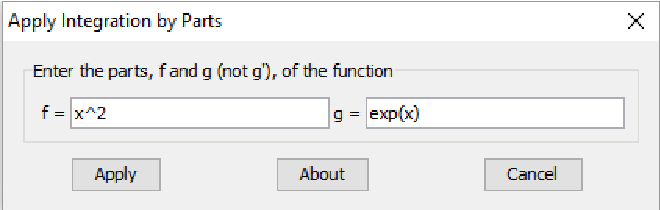
\includegraphics[width=0.6\textwidth]{tutorials/figures/IntTutorQ1-2-eps-converted-to.pdf}
\adjincludegraphics[width=0.8\textwidth,trim={0 {0.5\height} 0 0},clip]{tutorials/figures/IntTutorQ1-3-eps-converted-to.pdf}
\end{figure}

\begin{figure}[h]
\caption{Using the constant multiple rule, integration by parts a second time, and the exponential rule to evaluate the integral.}
\centering
\adjincludegraphics[width=0.8\textwidth,trim={0 {0.2\height} 0 0},clip]{tutorials/figures/IntTutorQ1-4-eps-converted-to.pdf}\\
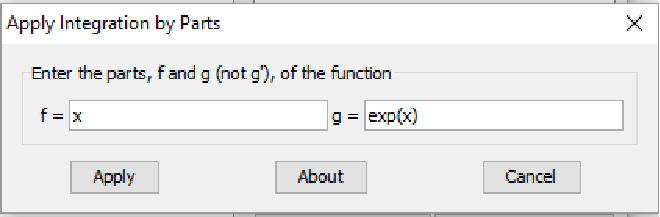
\includegraphics[width=0.6\textwidth]{tutorials/figures/IntTutorQ1-5-eps-converted-to.pdf}
\adjincludegraphics[width=0.8\textwidth,trim={0 {0.2\height} 0 0},clip]{tutorials/figures/IntTutorQ1-6-eps-converted-to.pdf}\\
\end{figure}

\clearpage

\subsection{Evaluating $\displaystyle\int_{-\pi/2}^{\pi/4} x\sin(x^2+1)$ Using Substitution}

\index{integral!integration methods tutor}

\begin{figure}[h]
\caption{If you use the All Steps button, then Maple will evaluate the integral, showing all steps.}
\centering
\adjincludegraphics[width=0.8\textwidth,trim={0 0 0 0},clip]{tutorials/figures/IntTutorQ2-eps-converted-to.pdf}\\
\end{figure}

\clearpage

\section{Volumes of Revolution}
\label{sec:volume_of_revolution_tutor}

\index{volume of revolution!tutor}
\index{packages!Student[Calculus1]}

The Volume of Revolution tutor is used to evaluate the volume of a solid obtained by rotating a region about a specified horizontal or vertical axis.

\begin{figure}[h]
\caption{Opening up the Volume of Revolution tutor using menus.}
\centering
\adjincludegraphics[width=\textwidth]{tutorials/figures/VoRTutorLoad1-eps-converted-to.pdf}
\end{figure}

\begin{figure}[h]
\caption{Opening up the Volume of Revolution tutor using commands. The \texttt{Student[Calculus1]} package is required.}
\centering
\adjincludegraphics[width=\textwidth]{tutorials/figures/VoRTutorLoad2-eps-converted-to.pdf}
\end{figure}

\newpage

\subsection{Volume Obtained by Rotating the Region Bounded by the Parabolas $y=x^2-4$ and $y=-x^2+4$ about $y=2$}

\index{plot!multiple functions}
\index{plot!axes intervals}
\index{volume of revolution!tutor}

It is a good idea to begin by plotting the two-dimensional regions to find the intersection points of the two curves.

\begin{maplegroup}
\begin{mapleinput}
\mapleinline{active}{1d}{plot([-x\symbol{94}2+4, x\symbol{94}2-4], x=-2..2);
}{}
\end{mapleinput}
\mapleresult
\mapleplot{tutorials/figures/volumeofrevolutionplot2d1-eps-converted-to.pdf}
\end{maplegroup}

In the Volume of Revolution Tutor, be sure to enter the functions, the interval for the variable, and the information about the axis of revolution.

\begin{figure}
\caption{Setting the Volume of Revolution tutor to revolve the region about a horizontal axis.}
\centering
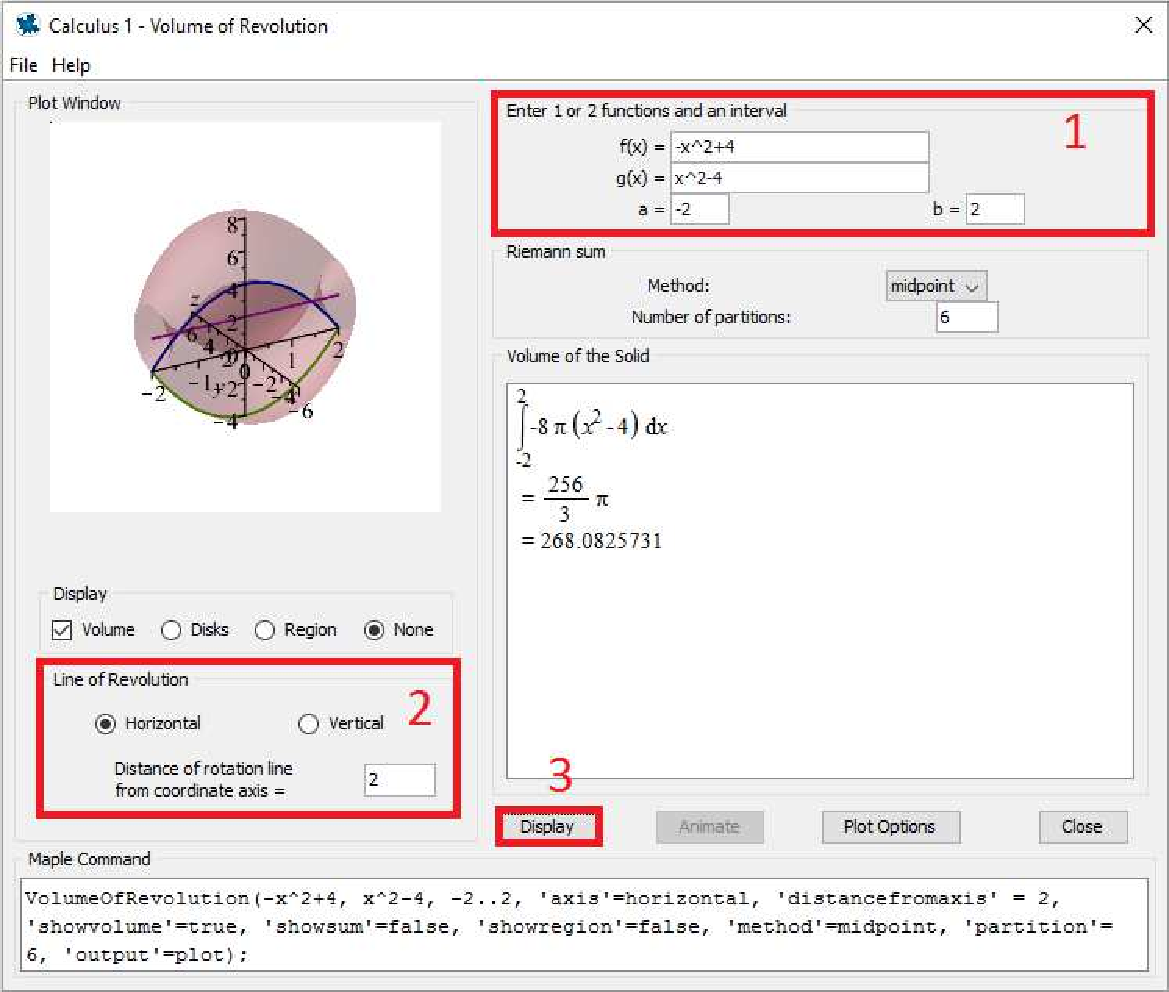
\includegraphics[width=0.9\textwidth]{tutorials/figures/VoRTutorQ1-1-eps-converted-to.pdf}
\end{figure}

\marginnote[-4cm]{When typing in the functions in the tutor, you will not have access to the palettes toolbar in Maple. You will need to type out commands such as \texttt{sqrt()} for square roots. You must also include the symbol * for multiplication.}

The Maple Command at the bottom of the tutor can be copied and pasted into a new Maple input in your worksheet. You can then change the various options in that command to output the plot of the solid, the integral used to obtain the volume, or the numerical value of the volume.

\begin{maplegroup}
\begin{mapleinput}
\mapleinline{active}{1d}{with(Student[Calculus1]):
}{}
\end{mapleinput}
\end{maplegroup}

\marginnote[1cm]{Using the output from the Volume of Revolution Tutor and changing the \texttt{output} option will let you display the region, the value of the volume, and the integral used to obtain the volume.}

\begin{maplegroup}
\begin{mapleinput}
\mapleinline{active}{1d}{VolumeOfRevolution(-x\symbol{94}2+4, x\symbol{94}2+4, -2..2, 'axis'=horizontal, 'distancefromaxis' = 0, 'showvolume'=true, 'showsum'=false, 'showregion'=false, 'method'=midpoint, 'partition'= 6, 'output'=plot);
}{}
\end{mapleinput}
\mapleresult
%\mapleplot{tutorials/figures/volumeofrevolutionplot3d1-eps-converted-to.pdf}
\mapleplot{tutorials/figures/volumeofrevolutionplot3d1-eps-converted-to.png}
\end{maplegroup}

\begin{maplegroup}
\begin{mapleinput}
\mapleinline{active}{1d}{VolumeOfRevolution(-x\symbol{94}2+4, x\symbol{94}2+4, -2..2, 'axis'=horizontal, 'distancefromaxis' = 0, 'showvolume'=true, 'showsum'=false, 'showregion'=false, 'method'=midpoint, 'partition'= 6, 'output'=integral);
}{}
\end{mapleinput}
\mapleresult
\begin{maplelatex}
\mapleinline{inert}{2d}{Int(16*Pi*x^2, x = -2 .. 2)}{\[\displaystyle \int_{-2}^{2}\!16\,\pi\,{x}^{2}\,{\rm d}x\]}
\end{maplelatex}
\end{maplegroup}

\index{volume of revolution!tutor}

\begin{maplegroup}
\begin{mapleinput}
\mapleinline{active}{1d}{VolumeOfRevolution(-x\symbol{94}2+4, x\symbol{94}2+4, -2..2, 'axis'=horizontal, 'distancefromaxis' = 0, 'showvolume'=true, 'showsum'=false, 'showregion'=false, 'method'=midpoint, 'partition'= 6, 'output'=value);
}{}
\end{mapleinput}
\mapleresult
\begin{maplelatex}
\mapleinline{inert}{2d}{(256/3)*Pi}{\[\displaystyle {\frac {256\,\pi}{3}}\]}
\end{maplelatex}
\end{maplegroup}

\clearpage

\subsection{Volume Obtained by Rotating the Region Bounded by the Parabolas $y=x^2-4$ and $y=-x^2+4$ about $x=-3$}

In this case, we will revolve the same region as above, but around a vertical axis.

\index{volume of revolution!tutor}

\begin{figure}
\caption{Setting the Volume of Revolution tutor to revolve the region about a vertical axis.}
\centering
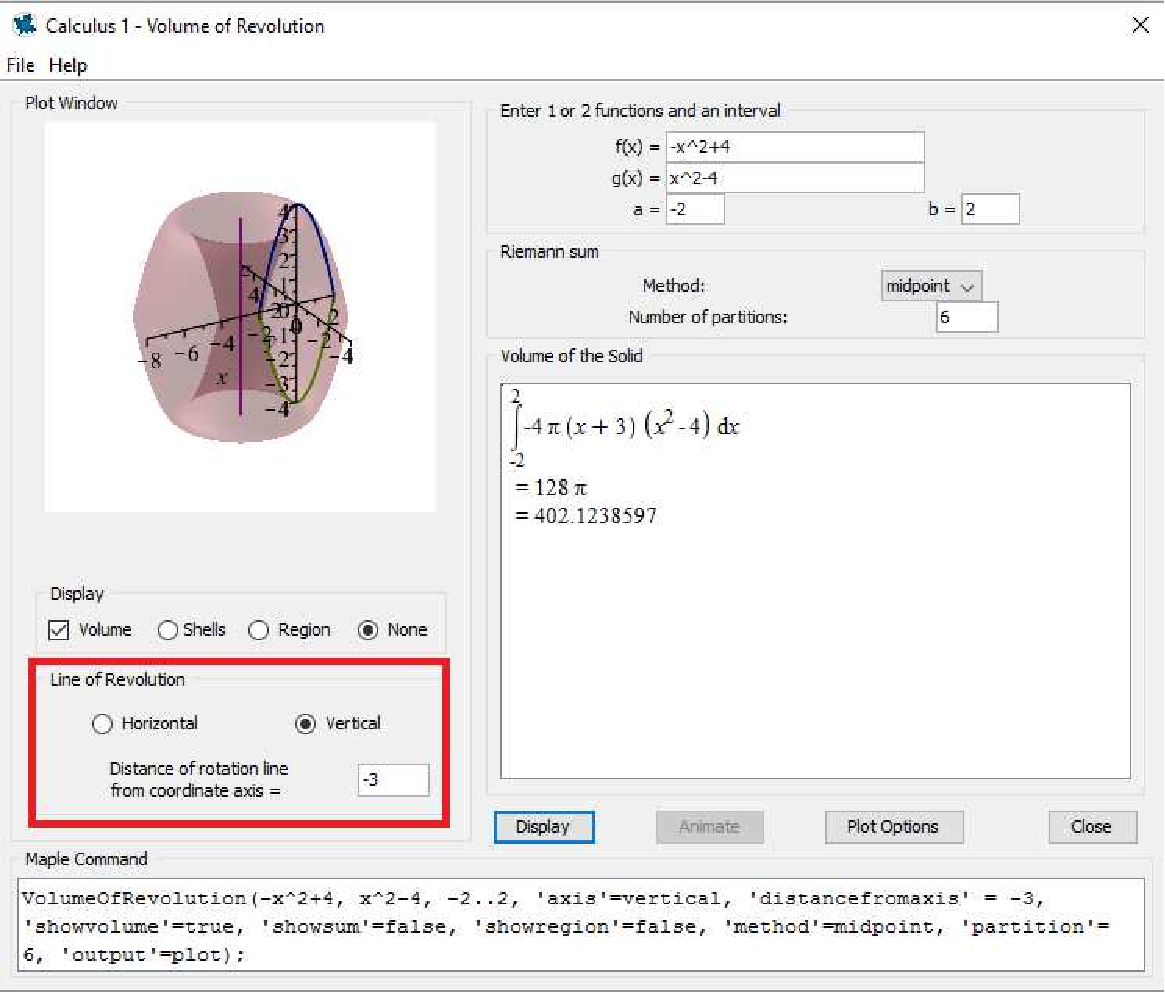
\includegraphics[width=0.9\textwidth]{tutorials/figures/VoRTutorQ1-2-eps-converted-to.pdf}
\end{figure}

\section{Arc Length}
We can use the \texttt{ArcLength()} command that is available in the \texttt{Student[Calculus1]} package to find the arc length of a function over a specified interval.

\index{packages!Student[Calculus1]}
\index{arc length}
\index{evalf}

\subsection{Arc Length of a Parabola}

\begin{maplegroup}
\begin{mapleinput}
\mapleinline{active}{1d}{with(Student[Calculus1]):
}{}
\end{mapleinput}
\end{maplegroup}

\begin{maplegroup}
\begin{mapleinput}
\mapleinline{active}{1d}{g(x) := x\symbol{94}2;
}{}
\end{mapleinput}
\mapleresult
\begin{maplelatex}
\mapleinline{inert}{2d}{g := proc (x) options operator, arrow; x^2 end proc}{\[\displaystyle g\, := \,x\mapsto {x}^{2}\]}
\end{maplelatex}
\end{maplegroup}

\begin{maplegroup}
\begin{mapleinput}
\mapleinline{active}{1d}{arcg := ArcLength(g(x), x=0..Pi);
}{}
\end{mapleinput}
\mapleresult
\begin{maplelatex}
\mapleinline{inert}{2d}{arcg := (1/2)*Pi*sqrt(4*Pi^2+1)-(1/4)*ln(-2*Pi+sqrt(4*Pi^2+1))}{\[\displaystyle {\it arcg}\, := \,1/2\,\pi \, \sqrt{4\,{\pi }^{2}+1}-1/4\,\ln  \left( -2\,\pi + \sqrt{4\,{\pi }^{2}+1} \right) \]}
\end{maplelatex}
\end{maplegroup}

\begin{maplegroup}
\begin{mapleinput}
\mapleinline{active}{1d}{evalf(arcg);
}{}
\end{mapleinput}
\mapleresult
\begin{maplelatex}
\mapleinline{inert}{2d}{10.62814707}{\[\displaystyle  10.62814707\]}
\end{maplelatex}
\end{maplegroup}
\clearpage
\subsection{Arc Length of a Sinusoid}

\index{mathematical functions!sine}

\begin{maplegroup}
\begin{mapleinput}
\mapleinline{active}{1d}{f(x) := sin(x);
}{}
\end{mapleinput}
\mapleresult
\begin{maplelatex}
\mapleinline{inert}{2d}{f := proc (x) options operator, arrow; sin(x) end proc}{\[\displaystyle f\, := \,x\mapsto \sin \left( x \right) \]}
\end{maplelatex}
\end{maplegroup}

\begin{maplegroup}
\begin{mapleinput}
\mapleinline{active}{1d}{arcf := ArcLength(f(x), x=0..Pi);
}{}
\end{mapleinput}
\mapleresult
\marginnote{\texttt{EllipticE()} is a special function in Maple that you don't have to know. We at least can evaluate it, however.}
\begin{maplelatex}
\mapleinline{inert}{2d}{arcf := 2*sqrt(2)*EllipticE((1/2)*sqrt(2))}{\[\displaystyle {\it arcf}\, := \,2\, \sqrt{2}{\it EllipticE} \left( 1/2\, \sqrt{2} \right) \]}
\end{maplelatex}
\end{maplegroup}

\begin{maplegroup}
\begin{mapleinput}
\mapleinline{active}{1d}{evalf(arcf);
}{}
\end{mapleinput}
\mapleresult
\begin{maplelatex}
\mapleinline{inert}{2d}{3.820197788}{\[\displaystyle  3.820197788\]}
\end{maplelatex}
\end{maplegroup}

\index{arc length}
\index{evalf}
\index{arc length!output=integral}


We can add the parameter \texttt{output = integral} to the \texttt{ArcLength()} command to display the integral for calculating the arc length.

\begin{maplegroup}
\begin{mapleinput}
\mapleinline{active}{1d}{ArcLength(f(x), x=0..Pi, output=integral);
}{}
\end{mapleinput}
\mapleresult
\begin{maplelatex}
\mapleinline{inert}{2d}{Int(sqrt(cos(x)^2+1), x = 0 .. Pi)}{\[\displaystyle \int _{0}^{\pi }\! \sqrt{ \left( \cos \left( x \right)  \right) ^{2}+1}\,\,{dx}\]}
\end{maplelatex}
\end{maplegroup}
